
Stress is defined a a force applied to an area, $\sigma = F/\ell^2$

\section{Elastic Tensor Notation}

The theory of elasticity is a generalization of Hooke's law which relates the force $F$ needed to extend or compress a spring scales linearly with the spring constant  $k$, and the change in the length of spring $\Delta x$.  Put together, Hooke's law states

\begin{equation}\label{eq:hooke_law}
    \bm{F} = -k \Delta x
\end{equation}
with the negative sign implying that restorive force is produced by the spring is in the direction opposite of $\bm{F}$.

%\begin{figure}[h]
%  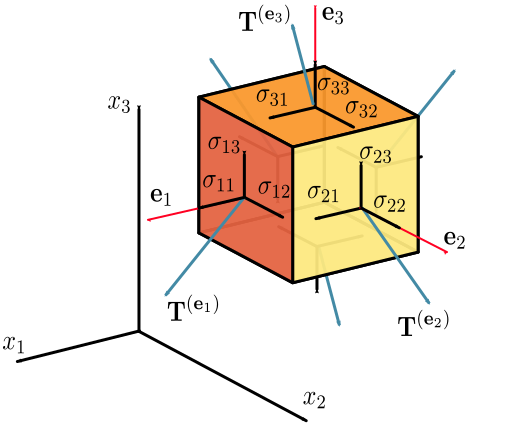
\includegraphics{stress_tensor}
%  \caption{Image by Sanpaz, distributed under a CC-BY-SA 3.0 license\cite{wiki2009_cauchy_tensor}}
%  \label{fig:stress_tensor}
%  \centering
%\end{figure}

To generalize Hookes law for application to solids, the force applied is a applied to vanishing small surface. There are nine components to the stress applied to a body as represented in the schematic\ref{fig:stress_tensor}, referred to as the Cauchy stress tensor\cite{timeshenko1970_elasticity},
\begin{equation}
  \sigma_{ij}
  =
  \begin{pmatrix}
    \sigma_{11} & \sigma{12} & \sigma{13} \\
    \sigma_{21} & \sigma{22} & \sigma{23} \\
    \sigma_{31} & \sigma{32} & \sigma{33}
  \end{pmatrix},
\end{equation}
the faces of the representational solid are oriented to the normal vectorwhere the normal stress, $\sigma_{ii} 
The Cauchy stress tensor, $\sigma_{ii}$, applied normal to the $\bm{e}_1$, is a normal pressure load.  Since the deformations are smalll then
\begin{equation}
  \sigma_{ii}=
\end{equation}

For a static body, the components of the Cauchy stress tensor in every material point in the body satisfies the Cauchy equations of motion for zero acceleration\cite{timeshenko1970_elasticity}, and the conservation of angular momentum implies that $\sigma_{ij}=\sigma{ji}$.

\begin{equation}
  \sigma_{ij} = C_{ijkl}\epsilon_{kl}
\end{equation}
where $\sigma_{ij}$ is the second order pressure tensor, and $\epsilon{kl}$ is a second order strain tensor.
$C_{ijkl}$ are the components of the fourth-order stiffness tensor of the material properties.  For three dimensions the fourth order has 81 components.
